% !TeX root = ../../../../../thesis.tex

%\subsubsection{230 V AC LED}
\subsubsection{LEDs powered directly by 230 V AC}


There also exists LED lighting fixture which work directly with AC, without having an external SMPS.
An example of such an LED can be seen in \autoref{fig:ac-commercial-230v-ac-led} \cite{commercial-230v-ac-led-aliexpress}.



For this LED it is investigated what the current signature looks like when the LED is constantly on, and when the LED is encoding information.
To measure the current, a 22 ohm resistor is placed in series with the light and the voltage drop over this resistor is measured.
Again, we are only looking at how the current signature behaves, at this point we are not interested in how much current is exactly being drawn.
In order to modulate the LED so that information is encoded in the current, changes had to be made to the internal hardware of the light fixture.
In \autoref{app:commercial-230v-ac-modified-schematic} a schematic can be found, which shows the original circuit and what was modified in order to modulate the LED.
The modifications made, include two transistors to switch the LEDs off and stop the capacitor from charging. 
With these transistors the entire current flow can be stopped thereby drawing zero current when we want to modulate a `0' symbol.
When a `1' symbol needs to be modulated, the transistors are turned on, and the LED behaves in a normal manner.
The transistors are controlled via a micro-controller through an optocoupler to protect the micro-controller in the development stages.



\begin{figure}[t]
	\centering     %%% not \center
	\subfigure[LED is constantly on. X-axis: 5 ms/div, Y-axis: 1 V/div.]{
		\label{fig:commercial-230v-ac-led-on-annotated}
		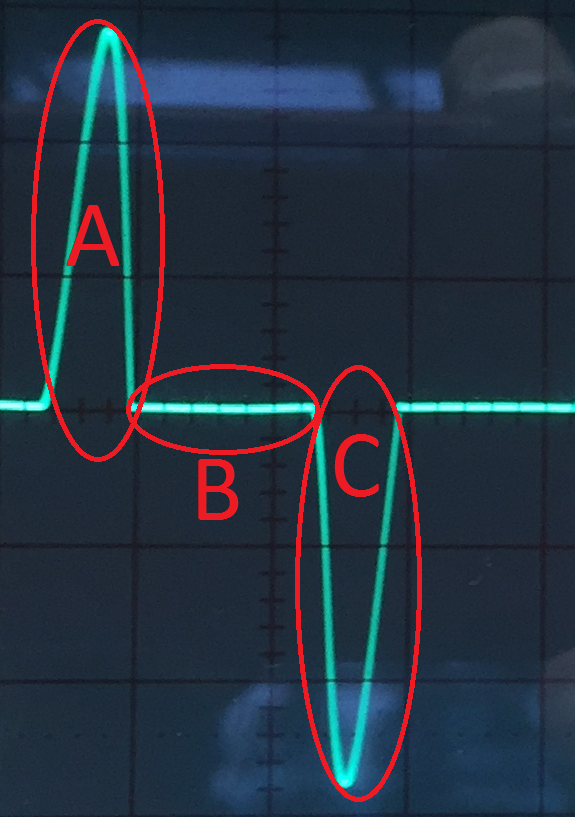
\includegraphics[angle=0,width=0.3\textwidth,keepaspectratio]
		{chapters/hardware-chapters/AC/ac-modulator/commercial-230v-ac-led/commercial-230v-ac-led-on-annotated.png}
	}
	\subfigure[LED is being modulated at 4 kHz. X-axis: 1 ms/div, Y-axis: 5 V/div.]{
		\label{fig:commercial-230v-ac-led-modulating}
		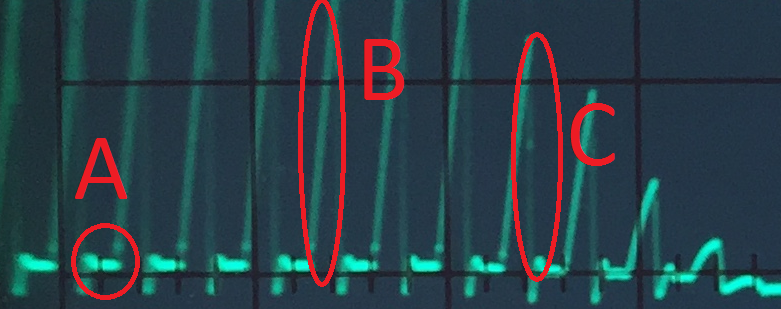
\includegraphics[angle=0,width=0.5\textwidth,keepaspectratio]
		{chapters/hardware-chapters/AC/ac-modulator/commercial-230v-ac-led/commercial-230v-ac-led-modulating-annotated.png}
	}

	\caption{Voltage measured over a 22 ohm series resistor at the primary side, to determine the current signature of a commercial 230 V AC LED.}
\end{figure}



When the LED is off, there is no current draw.
In Figure \ref{fig:commercial-230v-ac-led-on-annotated} the current signature can be seen when the LED is constantly on.
This figure shows 20 ms of the current signal, this is exactly one period of the supplied AC voltage: $t = \frac{1}{f} = \frac{1}{50} = 0.020$ s $= 20$ ms.
Every 20 ms this current draw repeats itself.
In the figure, three regions can be seen: A, B and C.
Each region will now be explained:

\begin{itemize}
	\item In region A, the supplied AC voltage is positive, and so the current that flows is positive.
	As can be seen from the schematic in \autoref{app:commercial-230v-ac-modified-schematic}, all the LEDs are connected in series.
	This means that a certain voltage is required in order for the LEDs to draw current.
	The required voltage is available at the start of region A and is no longer available at the end of region A and the current flow stops.
	The width of the peak is 4 ms.
	This is because in those 4 ms, there is enough voltage available to power all the LEDs in series. 
	The height of the peak indicates how much current is drawn.

	\item The start of region B starts when region A stops.
	The required voltage is no longer available and so the current flow stops and the LED no longer emits light.
	During this region there is no current flow.
	This is a good property: If the LED is off there is no current flow, exactly what we require.

	\item Region C starts when region B stops.
	At this point in time, there is enough voltage available for the LEDs to start drawing current again.
	But the voltage that is now available, is not positive as it was in region A, but is negative.
	That is why this peak goes the opposite direction of the peak seen in region A.
	The current that flows is in that case negative, because the voltage is also negative.
	In other aspects this peak has the same properties as those of the peak in region A, it has the same width and height.

\end{itemize}


Only in region A and C, the LED can be used to encode information.
Because in region B, the is no current draw and therefor we cannot modulate information.
The peaks in region A and C are both 4 ms wide.
This means that there is 8 ms of time available for modulation in the 20 ms period, so $\frac{8}{20} = 40$ \% of the time is available for encoding the ID with this LED.
To compare with a DC environment: In a DC scenario, the power supply always supplies a constant voltage, so the LED can always emit light and therefor can always draw current, so 100 \% of the time is available for modulation.
If the ID would have a certain length, it would take time $t$ to modulate this ID in a DC environment and time $2.5 \times t$ with this AC LED if the ID could not be transmitted inside the 4 ms window. 


Now that the current signature has been investigated when the LED is on, the LED will be now be turned on and off with a frequency of 4 kHz to investigate how the current signature behaves.
In Figure \ref{fig:commercial-230v-ac-led-modulating} the current signature can be seen when the LED is being modulated with a frequency of 4 kHz.
The entire figure takes place inside region A of Figure \ref{fig:commercial-230v-ac-led-on-annotated}.
If this figure would have been showed for region C of Figure \ref{fig:commercial-230v-ac-led-on-annotated}, the amplitudes would have been negative.
Again, there are three regions highlighted:

\begin{itemize}

	\item In region A, the data being encoded is a `0' and the current draw is also zero.
	As discussed this is a desired property.

	\item Region B shows the transition from the LED being off to the LED being on.
	The current does not go straight up, but instead a slope can be seen.
	This is not a desired property.
	A square wave is desired, this LED is producing a triangular wave.

	\item In region C, the transition from the LED being on to the LED being off can be seen.
	This time the current does go immediately to zero, which is a good property.
	Around region C another issue can be seen. 
	The amplitude of the current becomes lower and lower until region A of Figure \ref{fig:commercial-230v-ac-led-on-annotated} ends.
	This is also not a desirable property, the current should always be some constant value and not decreasing over time.

\end{itemize} 



From this investigation it can be concluded that this 230 V AC LED is not suitable to map the ID into the current signature which is desired.
And also the time that would be available for modulation is limited, because there are many LEDs in series which require a high voltage which is only available for a short amount of time.








